\subsection{Determinação do calor específico de um metal}

Como segundo experimento, iremos determinar o calor específico de um pedaço de metal desconhecido. Para fazer isso, precisaremos primeiro selecionar materiais com capacidades conhecidas a fim de poder ter uma forma para determinar tal calor específico.\\

O primeiro desses itens é o calorímetro estudado no experimento anterior. Ele servirá para isolarmos o nosso sistema do ambiente a fim de obter resultados mais precisos, reduzindo a quantidade de energia que é escapa. 

Com a capacidade térmica (C) já conhecida, podemos adicionar uma certa quantidade de água ($m_a$) lá dentro e esperar o equilíbrio térmico, que será monitorado por meio de um termômetro eletrônico, obtendo assim a primeira medida de temperatura ($T_1$).

\begin{figure}[H]
  \centering
  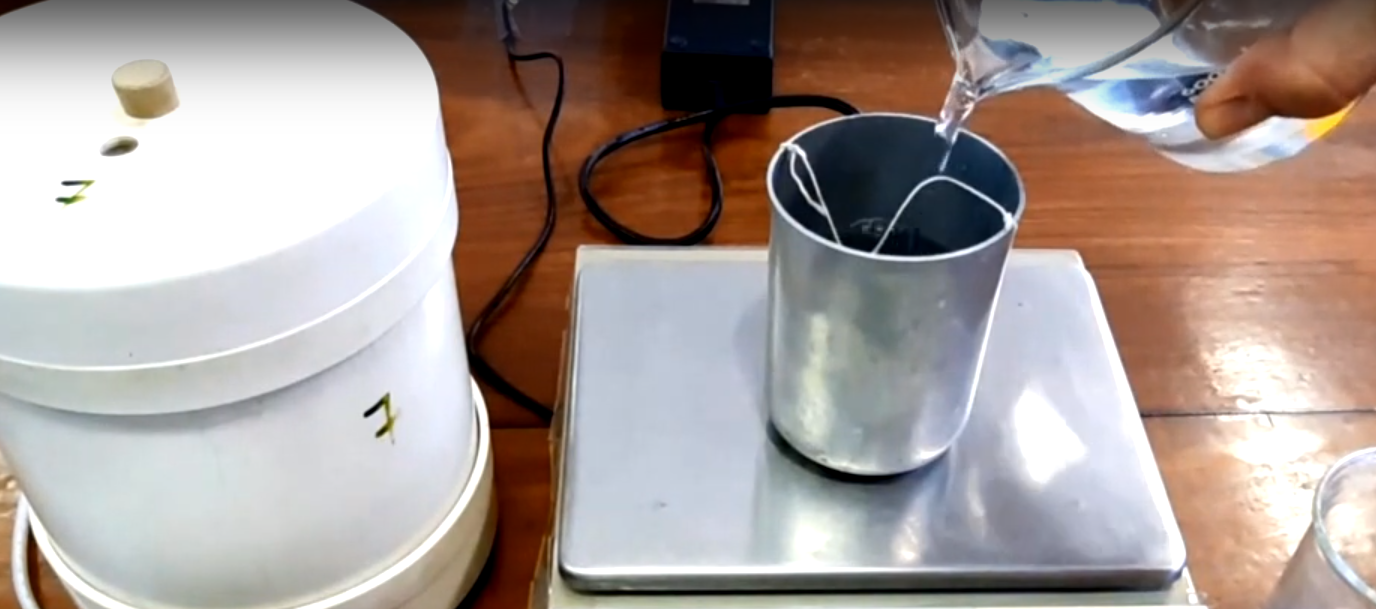
\includegraphics[scale=0.4]{images/agua-equilibrio-calorimetro.png}
  \caption{Calorímetro e o seu recipiente interior que entrará em equilíbrio com a água.}
\end{figure}

Em paralelo, colocamos o metal desconhecido dentro de um béquer com água e aquecemos esse conjunto até a fervura do líquido. Como sabemos que no momento da troca de fase a temperatura se torna constante, monitorando com um termômetro do mesmo tipo, aguardamos até esse valor estabilizar, obtendo assim a segunda medida da temperatura ($T_2$).\\

\begin{figure}[H]
  \centering
  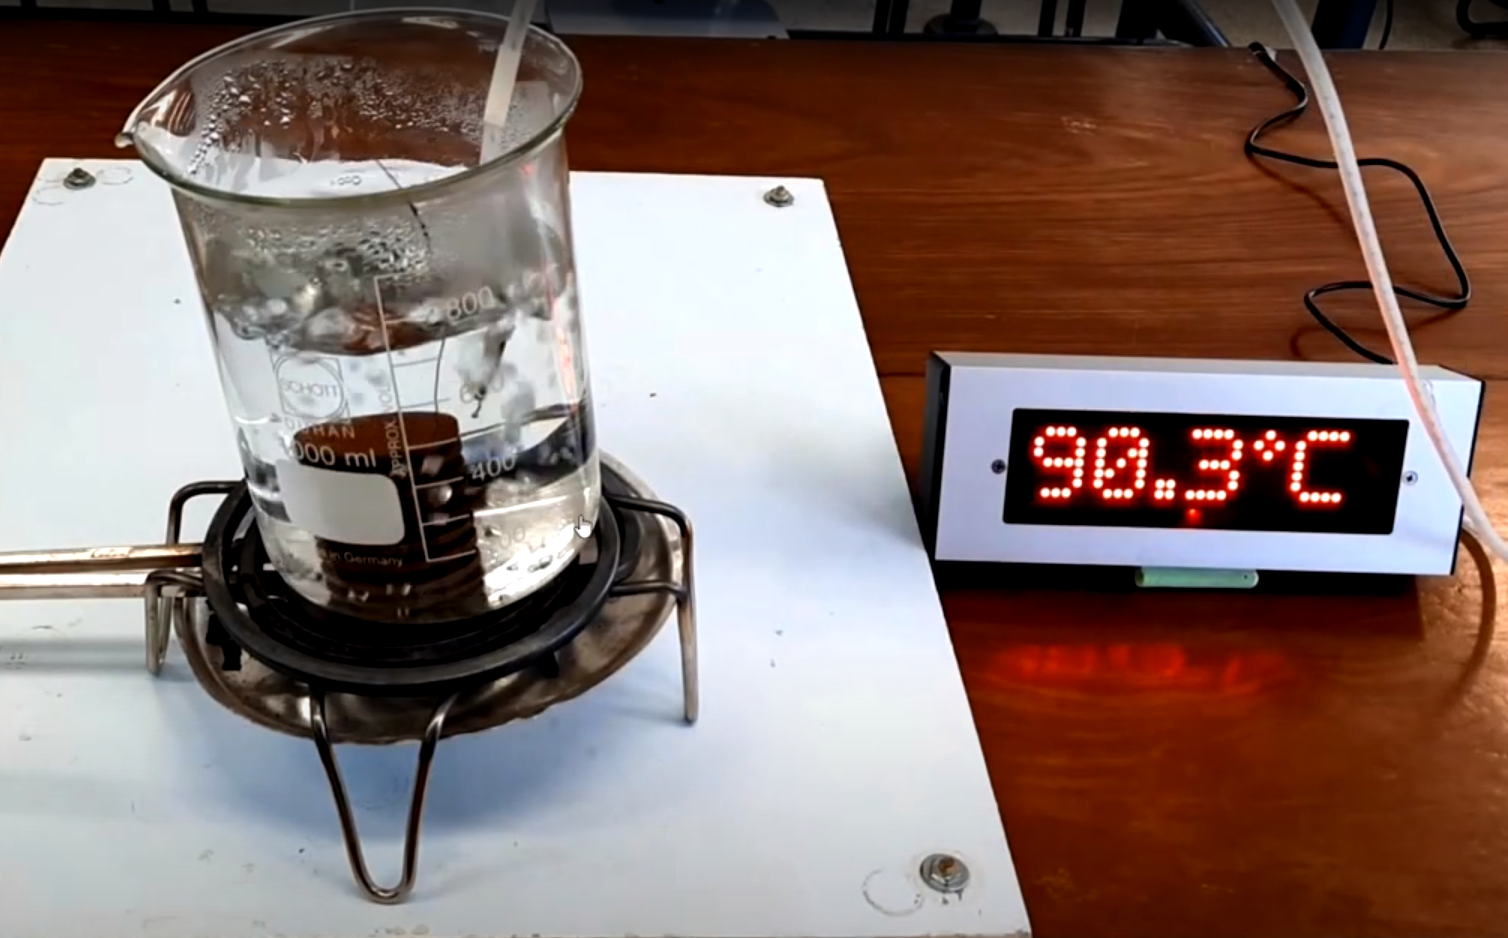
\includegraphics[scale=0.3]{images/fervura-dagua.png}
  \caption{Processo para esquentar o metal de forma uniforme utilizando a fervura da água.}
\end{figure}

Quando tudo estiver então anotado e pronto, o metal será retirado da fervura e rapidamente colocado dentro do calorímetro com água dentro. Esse processo fará com que os sistemas, antes separados, troquem calor entre si. Esse novo equilíbrio então será alcançado numa nova temperatura ($T_f$), que será a todo instante monitorada.\\

Dito tudo isso, podemos utilizar as equações de conservação de energia sabendo que esse sistema é praticamente isolado (a variação total de energia é nula):

\[ m_1 c_a (T_f - T_1) + m_2 c_m (T_f - T_2) + C (T_f - T_1) = 0 \]
\[ m_1 c_a \Delta T_{f1} + m_2 c_m \Delta T_{f2} + C \Delta T_{f1} = 0 \]

Ou seja, para determinar o calor específico do metal, basta um rearranjar essa expressão (já substituindo $c_a$ pois equivale 1 cal/g.ºC):

\begin{table}[H]
    \centering
    \begin{tabular}{ c||c  }
         $N = (m_1 + C) \cdot \Delta T_{f1}$ &
         $D = m_2 \cdot \Delta T_{f2}$
    \end{tabular}
\end{table}

\[ c_m = \frac{N}{D} \]

E sua incerteza:

\[ \delta N = [(m_1 + C) \cdot \delta \Delta T_{f1}] + [(\delta m_1 + \delta C) \cdot \Delta T_{f1}] \]

\[ \delta D = (\delta m_2 \cdot \Delta T_{f2}) + (m_2 \cdot \delta \Delta T_{f2}) \]

\[ \delta c_m = \frac{N \cdot \delta D + \delta N \cdot D}{D^2} \]

Dessa forma, conseguimos determinar o calor específico do metal desconhecido, e comparando com uma tabela de referencia encontrada online, é possível falar quem ele é.
